\section{The Marked Lambda Calculus}
\label{sec:calculus}

To begin to motivate the development of this section, consider \cref{fig:calculus-examples}, which
shows common type errors as they appear in the Hazel programming environment. These programs are
syntactically well-formed but ill-typed.
% For example, a simple error that may occur is the use of an free variable (\cref{fig:calculus-examples-free}).
% As in \cref{fig:calculus-examples-unbound}, the editor indicates that the usage of an free $y$ is
% invalid by highlighting it in red.

\begin{figure}[htbp]
  \begin{tabular}[b]{cc}
    \begin{subfigure}[b]{0.3\columnwidth}
      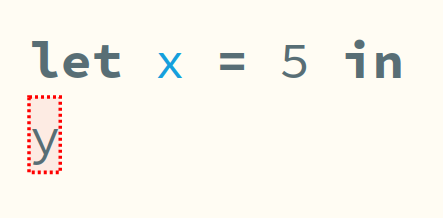
\includegraphics[width=\columnwidth]{images/haz3l-unbound-variable.png}
      \caption{Unbound variable error.}
      \label{fig:calculus-examples-unbound}
    \end{subfigure}
    &
    \begin{subfigure}[b]{0.3\columnwidth}
      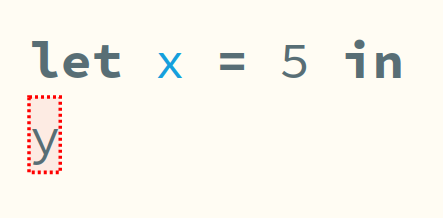
\includegraphics[width=\columnwidth]{images/haz3l-unbound-variable.png}
      \caption{Inconsistent types error.}
      \label{fig:calculus-examples-inconsistent-types}
    \end{subfigure} \\
    \begin{subfigure}[b]{0.3\columnwidth}
      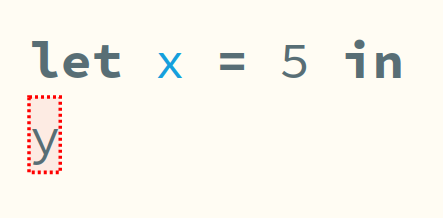
\includegraphics[width=\columnwidth]{images/haz3l-unbound-variable.png}
      \caption{Application of a non-lambda.}
      \label{fig:calculus-examples-app-non-lambda}
    \end{subfigure}
    &
    \begin{subfigure}[b]{0.3\columnwidth}
      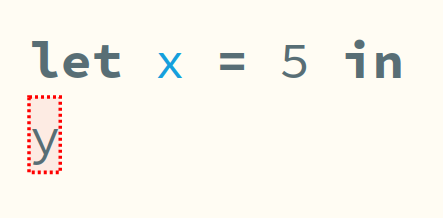
\includegraphics[width=\columnwidth]{images/haz3l-unbound-variable.png}
      \caption{Inconsistent branches error.}
      \label{fig:calculus-examples-inconsistent-branches}
    \end{subfigure}
  \end{tabular}
  %
  \caption{Examples of common type errors.}
  \label{fig:calculus-examples}
\end{figure}


% With local type inference, an expression might have a expected type. Consider
% \cref{fig:calculus-examples-inconsistent-types}, in which it is expected that both operands of the
% $+$ operator are numbers. Since $\textsf{true}$ is not a number, a type error arises, and Hazel
% indicates an inconsistency between the expected and actual types of the operand. The application in
% \cref{fig:calculus-examples-app-non-lambda} of a non-lambda leads to a similar kind of error. In
% this case, however, the expectation is not a singular type, but any member of a family of function
% types. \Cref{fig:calculus-examples-inconsistent-branches} presents an error caused by inconsistent
% branch types. As discussed in the introduction, Hazel opts to highlight the entire expression in such a situation,
% while other tools may choose one branch to be ``correct'' and ``blame'' the type mismatch error on
% the other.

The key contribution of this section is the \emph{marked lambda calculus}, a calculus based on the
gradually typed lambda calculus (GTLC) that formalizes the mechanism by which errors like these can
be localized, and how to recover, in all cases, from such errors. 
% In brief, the marked lambda calculus formalizes bidirectional type error localization with gradual
% recovery. 
\Cref{sec:calculus-calculus} introduces the syntax, judgemental structure, guiding metatheory, and
then goes through the rules, organized by syntactic form rather than judgement, to build intuition
about how the various judgements relate to one another.
All rules and theorems may be found organized by judgement form in the supplementary appendix for
reference, alongside a complete mechanization in the Agda proof assistant \cite{norell2007}
(discussed in \cref{sec:calculus-agda}).
We intentionally keep the marked lambda calculus minimal, because it is intended to capture the
essential idea and introduce a general pattern that language designers can employ to created marked
variants of their own type systems.
As an initial example, we consider a surprisingly subtle combination of features as a more
substantial case study: the combination of destructing let expressions with granular type
annotations, in \cref{sec:calculus-let}.
Finally, \cref{sec:calculus-polymorphism} briefly explores how the system might be extended to more
complex judgemental structures, such as parametric polymorphism.

\subsection{The Core Calculus}
\label{sec:calculus-calculus}

The marked lambda calculus is based on the gradually typed lambda calculus \cite{siek2006} extended
with numbers, booleans, pairs, and empty expression holes \cite{omar2017a}.
Given in \cref{fig:calculus-syntax}, the syntax consists of two expression languages:
%
\begin{itemize}
  \item The \emph{unmarked language}, which is the original language. Expressions of this language
    are called \emph{unmarked expressions}, denoted by the metavariable $\EMV$.

  \item The \emph{marked language}, which mirrors the structure of the unmarked language but is
    extended with \emph{error marks}. We call expressions of this language \emph{marked expressions},
    denoted $\ECMV$.
\end{itemize}
%
In this simple setting, we only need one sort for types, $\tau$. 
The base types $\TNum$ and $\TBool$ classify number and boolean
expressions. The number literal corresponding to the mathematical number $n$ is given by $\ENumMV$,
and there is a single arithmetic operation, addition. $\ETrue$ and
$\EFalse$ are the boolean values and
$\EIf{\EMV_1}{\EMV_2}{\EMV_3}$ is the boolean conditional. Arrow and product types classify lambda abstractions and pairs, respectively, in the usual way.

$\TUnknown$ is a type hole, which we identify with the unknown type from gradual type theory \cite{siek2006}.
Finally, to model the edit state of a program in development, $\EEHole$ denotes an \emph{empty expression hole},
used to represent syntactically incomplete portions of the program à la Hazelnut
\cite{omar2017b}. Note, however, that these empty expression holes are not at all semantically
critical to the calculus---they are included illustrate how the calculus fits into the larger
problem of modelling incomplete program states and to discuss polymorphic generalization in
\cref{sec:polymorphicGlobal}.

\begin{figure}[htbp]
  \[\begin{array}{rrcl}
      \TMName  & \TMV  & \Coloneqq & \TUnknown \mid \TNum \mid \TBool \mid \TArrow{\TMV}{\TMV} \mid \TProd{\TMV}{\TMV} \\
      \EMName  & \EMV  & \Coloneqq & x \mid \ELam{x}{\TMV}{\EMV} \mid \EAp{\EMV}{\EMV} \mid \ELet{x}{\EMV}{\EMV}
                         \mid           \ENumMV \mid \EPlus{\EMV}{\EMV} \\
               &       & \mid         & \ETrue \mid \EFalse \mid \EIf{\EMV}{\EMV}{\EMV}
                         \mid           \EPair{\EMV}{\EMV}
                         \mid           \EProjL{\EMV} \mid \EProjR{\EMV}
                         \mid           \EEHole \\
      \ECMName & \ECMV & \Coloneqq & x \mid \ECLam{x}{\TMV}{\ECMV} \mid \ECAp{\ECMV}{\ECMV} \mid \ECLet{x}{\ECMV}{\ECMV}
                         \mid           \ECNumMV \mid \ECPlus{\ECMV}{\ECMV} \\
               &       & \mid         & \ECTrue \mid \ECFalse \mid \ECIf{\ECMV}{\ECMV}{\ECMV}
                         \mid           \ECPair{\ECMV}{\ECMV} \mid \ECProjL{\ECMV} \mid \ECProjR{\ECMV}
                         \mid           \ECEHole \\
               &       & \mid         & \ECFree{x} \mid \ECInconType{\ECMV} \\
               &       & \mid         & \ECLamInconAsc{x}{\TMV}{\ECMV} \mid \ECLamAnaNonMatchedArrow{x}{\TMV}{\ECMV} \mid \ECApSynNonMatchedArrow{\ECMV}{\ECMV} \\
               &       & \mid         & \ECInconBr{\ECMV}{\ECMV}{\ECMV} \\
               &       & \mid         & \ECPairAnaNonMatchedProd{\ECMV}{\ECMV} \mid \ECProjLSynNonMatchedProd{\ECMV} \mid \ECProjRSynNonMatchedProd{\ECMV}
  \end{array}\]
  \caption{Syntax of the marked lambda calculus.}
  \label{fig:calculus-syntax}
\end{figure}

The key operation is \emph{marking}, which transforms an unmarked expression into a marked expression,
inserting error marks where appropriate.
This corresponds to a type checking
process with error localization and recovery. The marked language may then serve as a foundation for
other semantic services, such as constraint-based inference (as discussed in
\cref{sec:thi}). 
Intuitively, each of the mark forms corresponds to a different kind of error message that might be shown by an editor or emitted by a compiler. Note that we do not specify what the error message should say in this paper.

Throughout the remainder of this section, as we formulate marking for the GTLC, we will motivate and
give precise semantics for each error mark. Furthermore, when the core is extended, new marks may be needed, as we discuss below.
As we shall see, the rules for marking may be systematically derived by considering the error cases, yielding a recipe for developing error localization and recovery semantics for gradual, bidirectional type systems in general.

Before giving any of the rules, let us summarize the overall judgemental structure of the calculus. Note that colors in the judgement forms below are entirely redundant reading aids---color has no semantic significance.

As our starting point, types classify unmarked expressions by a completely standard \emph{bidirectional type system} \cite{dunfield2019,pierce2000}, which employs
two mutually defined judgments. \emph{Type synthesis}, written $\ctxSynTypeU{\ctx}{\EMV}{\TMV}$,
establishes that, under the typing context $\ctx$, the expression $e$ synthesizes or locally infers the type $\TMV$. \emph{Type analysis}, written $\ctxAnaTypeU{\ctx}{\EMV}{\TMV}$,
states that the expression $\EMV$ may appear where an expression of type $\TMV$ is expected.

The marked language possesses its own type system, also formulated bidirectionally. We write
$\ctxSynTypeM{\ctx}{\ECMV}{\TMV}$ for synthesis and $\ctxAnaTypeM{\ctx}{\ECMV}{\TMV}$ for analysis (in addition to the color difference, note the subscript on the turnstile to distinguish marked from unmarked typing). 

Finally, the \emph{marking} judgment is also of bidirectional nature. The synthetic marking judgment
$\ctxSynFixedInto{\ctx}{\EMV}{\ECMV}{\TMV}$ establishes that, under the context $\Gamma$, the
unmarked expression $\EMV$ is ``marked into'' the marked expression $\ECMV$, which synthesizes type
$\TMV$. Analogously, the analytic marking judgment $\ctxAnaFixedInto{\ctx}{\EMV}{\ECMV}{\TMV}$
states that $\EMV$ is marked into $\ECMV$, which analyzes against $\TMV$.

How can we ensure that the marking procedure is correctly defined? There are two critical
metatheorems that guide us as we continue. The first is a \emph{totality} of marking:
%
\begin{theorem}[name=Marking Totality] \
  \label{thm:calculus-marking-totality}
  \begin{enumerate}
    \item For all $\ctx$ and $\EMV$, there exist $\ECMV$ and $\TMV$ such that
      $\ctxSynFixedInto{\ctx}{\EMV}{\ECMV}{\TMV}$ and  $\ctxSynTypeM{\ctx}{\ECMV}{\TMV}$.
    \item For all $\ctx$, $\EMV$, and $\TMV$, there exists $\ECMV$ such that
      $\ctxAnaFixedInto{\ctx}{\EMV}{\ECMV}{\TMV}$ and $\ctxAnaTypeM{\ctx}{\ECMV}{\TMV}$.
  \end{enumerate}
\end{theorem}
%
That is, we may mark \emph{any} syntactically well-formed program in any context, resulting in a \emph{well-typed} marked program.


Furthermore, since error marks are effectively annotations on top of the program, marking should
preserve syntactic structure modulo those marks. \cref{fig:calculus-mark-erasure} gives part of the definition of \emph{mark erasure}, which converts marked expressions back into unmarked ones by
removing error marks. 
\begin{figure}[htbp]
  \newcommand{\erasesToRow}[2]{\erase{#1} & = & #2}
  \[\begin{array}{rcl}
    % \erasesToRow{\ECEHole}{\EEHole} \\
    \erasesToRow{x}{x} \\
    \erasesToRow{(\ECLam{x}{\TMV}{\ECMV})}{\ELam{x}{\TMV}{(\erase{\ECMV})}} \\
    \erasesToRow{(\ECAp{\ECMV_1}{\ECMV_2})}{\EAp{(\erase{\ECMV_1})}{(\erase{\ECMV_2})}} \\
    % \erasesToRow{(\ECLet{x}{\ECMV_1}{\ECMV_2})}{\ELet{x}{(\erase{\ECMV_1})}{(\erase{\ECMV_2})}} \\
    \erasesToRow{\ECNumMV}{\ENumMV} \\
    \erasesToRow{(\ECPlus{\ECMV_1}{\ECMV_2})}{\EPlus{(\erase{\ECMV_1})}{(\erase{\ECMV_2})}} \\
    \erasesToRow{\ECTrue}{\ETrue} \\
    \erasesToRow{\ECFalse}{\EFalse} \\
    \erasesToRow{(\ECIf{\ECMV_1}{\ECMV_2}{\ECMV_3})}{\EIf{(\erase{\ECMV_1})}{(\erase{\ECMV_2})}{(\erase{\ECMV_3})}} \\
    \erasesToRow{\ECUnbound{x}}{x} \\
    \erasesToRow{\ECInconType{\ECMV}}{\erase{\ECMV}} \\
    \erasesToRow{\ECInconBr{\ECMV_1}{\ECMV_2}{\ECMV_3}}{\EIf{(\erase{\ECMV_1})}{(\erase{\ECMV_2})}{(\erase{\ECMV_3})}} \\
  \end{array}\]
  %
  \caption{Mark erasure definition.}
  \label{fig:calculus-mark-erasure}
\end{figure}


Then, \cref{thm:calculus-marking-well-formedness} provides the necessary
\emph{well-formedness} criterion for marking.
%
\begin{theorem}[name=Marking Well-Formedness] \
  \label{thm:calculus-marking-well-formedness}
  \begin{enumerate}
    \item If $\ctxSynFixedInto{\ctx}{\EMV}{\ECMV}{\TMV}$,
      then $\ctxSynTypeM{\ctx}{\ECMV}{\TMV}$
        and $\erasesTo{\ECMV}{\EMV}$.
    \item If $\ctxAnaFixedInto{\ctx}{\EMV}{\ECMV}{\TMV}$,
      then $\ctxAnaTypeM{\ctx}{\ECMV}{\TMV}$
        and $\erasesTo{\ECMV}{\EMV}$.
  \end{enumerate}
\end{theorem}
%

Together, these metatheorems imply that to go from a standard bidirectional system for the unmarked language to a marking system, we need to handle all possible failure modes with appropriate marks and marking logic (otherwise totality would be violated) and without otherwise changing the program (otherwise well-formedness would be violated). Now, let us consider each form in turn.

\subsubsection{Numbers}
\label{sec:calculus-numbers}

To start, consider the simple case of numbers. Because of \emph{subsumption}, which is
discussed in more detail next, we need only define a synthesis rule for unmarked numbers, in which
number literals synthesize the type $\TNum$:
%
\begin{mathpar}
  \judgment{ }{
    \ctxSynTypeU{\ctx}{\ENumMV}{\TNum}
  }{USNum}
\end{mathpar}

How should numbers be marked? Straightforwardly, we simply give the same number as a marked
expression, synthesizing again $\TNum$. No type errors may occur in a just single number, so we only need
the following rules for marking numbers and typing the results: 
%
\begin{mathpar}
  \judgment{
  }{
    \ctxSynFixedInto{\ctx}{\ENumMV}{\ECNumMV}{\TNum}
  }{MKSNum}

  \judgment{ }{
    \ctxSynTypeM{\ctx}{\ECNumMV}{\TNum}
  }{MSNum}
\end{mathpar}

For addition expressions, the type of both operands should be $\TNum$. To denote this in a
bidirectional system, they are analyzed against $\TNum$, giving the following typing rule for
unmarked addition expressions:
%
\begin{mathpar}
  \judgment{
    \ctxAnaTypeU{\ctx}{\EMV_1}{\TNum} \\
    \ctxAnaTypeU{\ctx}{\EMV_2}{\TNum}
  }{
    \ctxSynTypeU{\ctx}{\EPlus{\EMV_1}{\EMV_2}}{\TNum}
  }{USPlus}
\end{mathpar}

The marking rule parallels \textsc{USPlus} closely. Since an expected type for each operand is known,
we shift the responsibility for any type errors to them. Hence, we recursively mark each operand in
analytic mode and rebuild the marked addition expression. The typing rule for marked addition
expressions then mirrors \textsc{USPlus} exactly.
%
\begin{mathpar}
  \judgment{
    \ctxAnaFixedInto{\ctx}{\EMV_1}{\ECMV_1}{\TNum} \\
    \ctxAnaFixedInto{\ctx}{\EMV_2}{\ECMV_2}{\TNum}
  }{
    \ctxSynFixedInto{\ctx}{\EPlus{\EMV_1}{\EMV_2}}{\ECPlus{\ECMV_1}{\ECMV_2}}{\TNum}
  }{MKSPlus}

  \judgment{
    \ctxAnaTypeM{\ctx}{\ECMV_1}{\TNum} \\
    \ctxAnaTypeM{\ctx}{\ECMV_2}{\TNum}
  }{
    \ctxSynTypeM{\ctx}{\ECPlus{\ECMV_1}{\ECMV_2}}{\TNum}
  }{MSPlus}
\end{mathpar}

\subsubsection{Subsumption}
\label{sec:calculus-subsumption}

Only synthetic rules are necessary for typing numbers and addition because of \emph{subsumption},
given below, which states that if an expression synthesizes a type, it may also be analyzed against
that type or any consistent type.
\[%
  \judgment{
    \ctxSynTypeU{\ctx}{\EMV}{\TMV'} \\
    \consistent{\TMV}{\TMV'} \\
    \subsumable{\EMV}
  }{
    \ctxAnaTypeU{\ctx}{\EMV}{\TMV}
  }{UASubsume}
\]%
We rely on the notion of \emph{type consistency} from gradual type theory, which defines a reflexive
and symmetric (but not transitive) relation between types, writing $\consistent{\TMV_1}{\TMV_2}$ to
mean that $\TMV_1$ is consistent with $\TMV_2$. Defined in \cref{fig:calculus-consistency}, this
replaces the notion of \emph{type equality} to relate the unknown type to all other types.

\begin{figure}[htbp]
  \raggedright
  \judgbox{\ensuremath{\consistent{\TMV_1}{\TMV_2}}} $\TMV_1$ is consistent with $\TMV_2$
  %
  \begin{mathpar}
    \judgment{ }{
      \consistent{\TUnknown}{\TMV}
    }{TCUnknown1}

    \judgment{ }{
      \consistent{\TMV}{\TUnknown}
    }{TCUnknown2}

    \judgment{ }{
      \consistent{\TMV}{\TMV}
    }{TCRefl}

    \judgment{
      \consistent{\TMV_1}{\TMV_1'} \\
      \consistent{\TMV_2}{\TMV_2'} \\
    }{
      \consistent{\TArrow{\TMV_1}{\TMV_2}}{\TArrow{\TMV_1'}{\TMV_2'}}
    }{TCArr}

    \inferrule[TCProd]{
      \consistent{\TMV_1}{\TMV_1'} \\
      \consistent{\TMV_2}{\TMV_2'} \\
    }{
      \consistent{\TProd{\TMV_1}{\TMV_2}}{\TProd{\TMV_1'}{\TMV_2'}}
    }
  \end{mathpar}
  \vspace{-10px}
  \caption{Type consistency.}
  \label{fig:calculus-consistency}
\end{figure}

Hence, when checking $\ENumMV$ against a known expected type, subsumption checks that the type is
consistent with $\TNum$, the type that $\ENumMV$ synthesizes. This succeeds for $\TUnknown$ and
$\TNum$.

We also restrict the usage of subsumption to ``subsumable'' syntactic forms, written
$\subsumable{\EMV}$. This judgment is defined for all syntactic forms except lambda abstractions,
conditionals, and pairs, the only ones with both synthesis and analysis rules (see below). In other words, we restrict subsumption to
be the rule of ``last resort'', which is necessary to establish that marking and typing are
deterministic (see \cref{thm:calculus-marking-unicity}).

Now, to define analytic marking on forms without explicit analytic typing rules, we also need
subsumption rules for marking and marked expression typing. Note that we define an analogous notion
of ``subsumability'' for marked expressions, written $\subsumable{\ECMV}$.
%
\begin{mathpar}
  \judgment{
    \ctxSynFixedInto{\ctx}{\EMV}{\ECMV}{\TMV'} \\
    \consistent{\TMV}{\TMV'} \\
    \subsumable{\EMV}
  }{
    \ctxAnaFixedInto{\ctx}{\EMV}{\ECMV}{\TMV}
  }{MKASubsume}

  \judgment{
    \ctxSynTypeM{\ctx}{\ECMV}{\TMV'} \\
    \consistent{\TMV}{\TMV'} \\
    \subsumable{\ECMV}
  }{
    \ctxAnaTypeM{\ctx}{\ECMV}{\TMV}
  }{MASubsume}
\end{mathpar}

But what happens when the synthesized type of an expression is \emph{not} consistent with the
expected type, i.e. that the premise $\consistent{\TMV}{\TMV'}$ fails? Recalling the example of
\cref{fig:calculus-examples-inconsistent-types}, subsumption would be used to analyze $\ETrue$
against $\TNum$ when checking $\EPlus{\ETrue}{1}$, which fails since $\inconsistent{\TNum}{\TBool}$, i.e.
\textsc{UASubsume} does not apply. At this point, traditional typing semantics would simply fail the type
checking process. \textsc{MKASubsume} would also not be applicable, leaving marking
undefined in those cases.

To satisfy marking totality, such a possibility motivates an \emph{inconsistent type mark}
$\ECInconType{\ECMV}$, which is applied when the synthesized type of $\ECMV$ is inconsistent
with the expected type:
%
\begin{mathpar}
  \judgment{
    \ctxSynFixedInto{\ctx}{\EMV}{\ECMV}{\TMV'} \\
    \inconsistent{\TMV}{\TMV'} \\
    \subsumable{\EMV}
  }{
    \ctxAnaFixedInto{\ctx}{\EMV}{\ECInconType{\ECMV}}{\TMV}
  }{MKAInconsistentTypes}

  \judgment{
    \ctxSynTypeM{\ctx}{\ECMV}{\TMV'} \\
    \inconsistent{\TMV}{\TMV'} \\
    \subsumable{\ECMV}
  }{
    \ctxAnaTypeM{\ctx}{\ECInconType{\ECMV}}{\TMV}
  }{MAInconsistentTypes}
\end{mathpar}
%
Observe that the premises of \textsc{MKAInconsistentTypes} are identical to those of
\textsc{MKASubsume}, except that $\inconsistent{\TMV}{\TMV'}$. By marking an error, the type checking process may carry on and provide semantic feedback for the rest of the program.

\subsubsection{Variables}
\label{sec:calculus-variables}

Let us now consider the case of variables. Typing in the unmarked language is standard, and because
of subsumption, only a synthetic rule is required:
\[%
  \judgment{
    \inCtx{\ctx}{x}{\TMV}
  }{
    \ctxSynTypeU{\ctx}{x}{\TMV}
  }{USVar}
\]%
That is, if $x$ is bound to a type in the typing context, it synthesizes that type.
Straightforwardly, marking converts an unmarked variable into the same variable via the following
rules:
%
\begin{mathpar}
  \judgment{
    \inCtx{\ctx}{x}{\TMV}
  }{
    \ctxSynFixedInto{\ctx}{x}{x}{\TMV}
  }{MKSVar}

  \judgment{
    \inCtx{\ctx}{x}{\TMV}
  }{
    \ctxSynTypeM{\ctx}{x}{\TMV}
  }{MSVar}
\end{mathpar}

However, consider the case that a variable, such as $y$ in \cref{fig:calculus-examples-free}, is \emph{not}
bound. Similar to above, \textsc{USVar} would not apply. A total marking procedure should, however, report the error and
continue, motivating a \emph{free variable mark} $\ECFree{x}$ and the accompanying rules:
%
\begin{mathpar}
  \judgment{
    \notInCtx{\ctx}{x}
  }{
    \ctxSynFixedInto{\ctx}{x}{\ECFree{x}}{\TUnknown}
  }{MKSFree}

  \judgment{
    \notInCtx{\ctx}{x}
  }{
    \ctxSynTypeM{\ctx}{\ECFree{x}}{\TUnknown}
  }{MSFree}
\end{mathpar}
%
A free variable is marked as such, and since nothing may be said about their types, we synthesize
the unknown type. As with the inconsistent type mark, this allows type checking to proceed, with
usage of the free variable permitted in any expression.

\subsubsection{Lambda Abstractions}
\label{sec:calculus-lambda-abstractions}

Unlike numbers and variables, there are explicit synthesis and analysis rules for unmarked lambda
abstractions. This is because expected input and output types are known, and we may verify that the
type annotation and body match them.
%
\begin{mathpar}
  \judgment{
    \ctxSynTypeU{\extendCtx{\ctx}{x}{\TMV_1}}{\EMV}{\TMV_2}
  }{
    \ctxSynTypeU{\ctx}{\ELam{x}{\TMV_1}{\EMV}}{\TArrow{\TMV_1}{\TMV_2}}
  }{USLam}

  \judgment{
    \matchedArrow{\TMV_3}{\TMV_1}{\TMV_2} \\
    \consistent{\TMV}{\TMV_1} \\
    \ctxAnaTypeU{\extendCtx{\ctx}{x}{\TMV}}{\EMV}{\TMV_2}
  }{
    \ctxAnaTypeU{\ctx}{\ECLam{x}{\TMV}{\EMV}}{\TMV_3}
  }{UALam}
\end{mathpar}
%
The synthesis rule is standard. Analysis employs the judgment $\matchedArrow{\TMV}{\TMV_1}{\TMV_2}$,
which establishes that $\TMV$ is a \emph{matched arrow type} \cite{cimini2016}, i.e. it may be
considered an arrow type. Defined in \cref{fig:calculus-matched-arrow}, this notion is purely a
technical mechanism to avoid duplication of rules related to arrow types \cite{siek2015}.

\begin{figure}[htbp]
  \raggedright
  \judgbox{\ensuremath{\matchedArrow{\TMV}{\TMV_1}{\TMV_2}}} $\TMV$ has matched arrow type $\TArrow{\TMV_1}{\TMV_2}$
  %
  \begin{mathpar}
    \judgment{ }{
      \matchedArrow{\TUnknown}{\TUnknown}{\TUnknown}
    }{TMAUnknown}

    \judgment{ }{
      \matchedArrow{\TArrow{\TMV_1}{\TMV_2}}{\TMV_1}{\TMV_2}
    }{TMAArr}
  \end{mathpar}
  \vspace{-10px}
  \caption{Matched arrow types.}
  \label{fig:calculus-matched-arrow}
\end{figure}

The synthesis rule for marking intuitively follows \textsc{USLam} closely. We recursively
mark the body with an extended context and construct a new marked lambda
abstraction:
%
\begin{mathpar}
  \judgment{
    \ctxSynFixedInto{\extendCtx{\ctx}{x}{\TMV_1}}{\EMV}{\ECMV}{\TMV_2}
  }{
    \ctxSynFixedInto{\ctx}{\ELam{x}{\TMV_1}{\EMV}}{\ELam{x}{\TMV_1}{\ECMV}}{\TArrow{\TMV_1}{\TMV_2}}
  }{MKSLam}

  \judgment{
    \ctxSynTypeM{\extendCtx{\ctx}{x}{\TMV_1}}{\ECMV}{\TMV_2}
  }{
    \ctxSynTypeM{\ctx}{\ECLam{x}{\TMV_1}{\ECMV}}{\TArrow{\TMV_1}{\TMV_2}}
  }{MSLam}
\end{mathpar}
%
Similarly, we construct corresponding analytic rules:
%
\begin{mathpar}
  \judgment{
    \matchedArrow{\TMV_3}{\TMV_1}{\TMV_2} \\
    \consistent{\TMV}{\TMV_1} \\\\
    \ctxAnaFixedInto{\extendCtx{\ctx}{x}{\TMV}}{\EMV}{\ECMV}{\TMV_2}
  }{
    \ctxAnaFixedInto{\ctx}{\ELam{x}{\TMV}{\EMV}}{\ECLam{x}{\TMV}{\ECMV}}{\TMV_3}
  }{MKALam1}

  \judgment{
    \matchedArrow{\TMV_3}{\TMV_1}{\TMV_2} \\
    \consistent{\TMV}{\TMV_1} \\\\
    \ctxAnaTypeM{\extendCtx{\ctx}{x}{\TMV}}{\ECMV}{\TMV_2}
  }{
    \ctxAnaTypeM{\ctx}{\ECLam{x}{\TMV}{\ECMV}}{\TMV_3}
  }{MALam1}
\end{mathpar}

However, recalling totality, we look again to the premises of \textsc{UALam} to see what type errors
may arise. First, what if $\TMV_3$ is not a matched arrow type? This would be the case if it were
$\TNum$, for example. The lambda abstraction's synthesized type would indeed be inconsistent with
the expected type, but this case is slightly distinct from that of the inconsistent types mark: the
lambda expression is in analytic position. Instead, we mark $\ECAnaNonMatchedArrow{\ECMV}$ to
indicate that an expression of the non-matched arrow type $\TMV_3$ was expected, but a lambda
abstraction was encountered.
%
\begin{mathpar}
  \judgment{
    \notMatchedArrow{\TMV_3} \\
    \ctxAnaFixedInto{\extendCtx{\ctx}{x}{\TMV}}{\EMV}{\ECMV}{\TUnknown}
  }{
    \ctxAnaFixedInto{\ctx}{\ELam{x}{\TMV}{\EMV}}{\ECLamAnaNonMatchedArrow{x}{\TMV}{\ECMV}}{\TMV_3}
  }{MKALam2}

  \judgment{
    \notMatchedArrow{\TMV_3} \\
    \ctxAnaTypeM{\extendCtx{\ctx}{x}{\TMV}}{\ECMV}{\TUnknown}
  }{
    \ctxAnaTypeM{\ctx}{\ECLamAnaNonMatchedArrow{x}{\TMV}{\ECMV}}{\TMV_3}
  }{MALam2}
\end{mathpar}
%
Though no expected output type is known, we still need to check and mark the body; it is thus
analyzed against the unknown type in \textsc{MKALam2}. It is possible to instead synthesize the
body, but we choose analysis so that the body is always in analytic mode. The guiding design
principle in this decision is is a notion of ``conservation of mode,'' but it is not critical to the
calculus.

Note that in this example language, the distinction from the inconsistent type mark is of reduced
significance---all expressions synthesize a type. However, the addition of unannotated lambda
abstractions, for example, would necessitate such a distinction.

Another error arises when $\matchedArrow{\TMV_3}{\TMV_1}{\TMV_2}$, but
$\inconsistent{\TMV}{\TMV_1}$, i.e. the actual type annotation for $x$ is inconsistent with the
expected input type. The \emph{inconsistent ascription mark} $\ECLamInconAsc{x}{\TMV}{\ECMV}$ indicates exactly this
error, and we add a final pair of analytic rules:
%
\begin{mathpar}
  \judgment{
    \matchedArrow{\TMV_3}{\TMV_1}{\TMV_2} \\
    \inconsistent{\TMV}{\TMV_1} \\\\
    \ctxAnaFixedInto{\extendCtx{\ctx}{x}{\TMV}}{\EMV}{\ECMV}{\TMV_2}
  }{
    \ctxAnaFixedInto{\ctx}{\ELam{x}{\TMV}{\EMV}}{\ECLamInconAsc{x}{\TMV}{\ECMV}}{\TMV_3}
  }{MKALam3}

  \judgment{
    \matchedArrow{\TMV_3}{\TMV_1}{\TMV_2} \\
    \inconsistent{\TMV}{\TMV_1} \\\\
    \ctxAnaTypeM{\extendCtx{\ctx}{x}{\TMV_1}}{\ECMV}{\TMV_2}
  }{
    \ctxAnaTypeM{\ctx}{\ECLamInconAsc{x}{\TMV}{\ECMV}}{\TMV_3}
  }{MALam3}
\end{mathpar}

\subsubsection{Applications}
\label{sec:calculus-applications}

In the unmarked language, only a synthesis rule is necessary for applications:
\[%
  \judgment{
    \ctxSynTypeU{\ctx}{\EMV_1}{\TMV} \\
    \matchedArrow{\TMV}{\TMV_1}{\TMV_2} \\
    \ctxAnaTypeU{\ctx}{\EMV_2}{\TMV_1}
  }{
    \ctxSynTypeU{\ctx}{\EAp{\EMV_1}{\EMV_2}}{\TMV_2}
  }{USAp}
\]%
Following the same methodology up to this point, we have the following marking and typing
rules:
%
\begin{mathpar}
  \judgment{
    \ctxSynFixedInto{\ctx}{\EMV_1}{\ECMV_1}{\TMV} \\
    \matchedArrow{\TMV}{\TMV_1}{\TMV_2} \\\\
    \ctxAnaFixedInto{\ctx}{\EMV_2}{\ECMV_2}{\TMV_1} \\
  }{
    \ctxSynFixedInto{\ctx}{\EAp{\EMV_1}{\EMV_2}}{\ECAp{\ECMV_1}{\ECMV_2}}{\TMV_2}
  }{MKSAp1}

  \judgment{
    \ctxSynTypeM{\ctx}{\ECMV_1}{\TMV} \\
    \matchedArrow{\TMV}{\TMV_1}{\TMV_2} \\\\
    \ctxAnaTypeM{\ctx}{\ECMV_2}{\TMV_1}
  }{
    \ctxSynTypeM{\ctx}{\ECAp{\ECMV_1}{\ECMV_2}}{\TMV_2}
  }{MSAp1}
\end{mathpar}

Again, to satisfy totality, we must consider the case when $\TMV$ is not a matched arrow type, such
as in the example of \cref{fig:calculus-examples-app-non-lambda}. There is no expected type for the
argument, so we perform analytic marking on $\EMV_2$ against the unknown type. In this case, it is
not quite right to mark $\EMV_1$ with the inconsistent type mark; rather than any single type, it is
any member of the family of arrow types that is expected. For such a ``constrained'' synthetic
mode, we use a specialized mark $\ECSynNonMatchedArrow{\ECMV}$, which indicates that $\ECMV$ was
expected to be a function---but was not. The output type is unknown, so the entire expression
synthesizes the unknown type.
%
\begin{mathpar}
  \judgment{
    \ctxSynFixedInto{\ctx}{\EMV_1}{\ECMV_1}{\TMV} \\
    \notMatchedArrow{\TMV} \\
    \ctxAnaFixedInto{\ctx}{\EMV_2}{\ECMV_2}{\TUnknown}
  }{
    \ctxSynFixedInto{\ctx}{\EAp{\EMV_1}{\EMV_2}}{\ECApSynNonMatchedArrow{\ECMV_1}{\ECMV_2}}{\TUnknown}
  }{MKSAp2}

  \judgment{
    \ctxSynTypeM{\ctx}{\ECMV_1}{\TMV} \\
    \notMatchedArrow{\TMV} \\
    \ctxAnaTypeM{\ctx}{\ECMV_2}{\TUnknown}
  }{
    \ctxSynTypeM{\ctx}{\ECApSynNonMatchedArrow{\ECMV}{\ECMV}}{\TUnknown}
  }{MSAp2}
\end{mathpar}

It is natural to extend this approach to other elimination forms that require the handling of
unmatched types, such as products. Indeed, the same approach is taken for projections below.
Another similar approach might indicate the same kind of error but mark the entire application.

\subsubsection{Booleans}
\label{sec:calculus-booleans}

The boolean values are similar to numbers: 
%
\begin{mathpar}
  \judgment{ }{
    \ctxSynTypeU{\ctx}{\ETrue}{\TBool}
  }{USTrue}

  \judgment{
  }{
    \ctxSynFixedInto{\ctx}{\ETrue}{\ECTrue}{\TBool}
  }{MKSTrue}

  \judgment{ }{
    \ctxSynTypeM{\ctx}{\ECTrue}{\TBool}
  }{MSTrue} \\

  \judgment{ }{
    \ctxSynTypeU{\ctx}{\EFalse}{\TBool}
  }{USFalse}

  \judgment{
  }{
    \ctxSynFixedInto{\ctx}{\EFalse}{\ECFalse}{\TBool}
  }{MKSFalse}

  \judgment{ }{
    \ctxSynTypeM{\ctx}{\ECFalse}{\TBool}
  }{MSFalse}
\end{mathpar}

Conditionals, however, present a more interesting case. In the unmarked language, we have both explicit
synthetic and analytic rules:
%
\begin{mathpar}
  \judgment{
    \ctxAnaTypeU{\ctx}{\EMV_1}{\TBool} \\
    \ctxSynTypeU{\ctx}{\EMV_2}{\TMV_1} \\\\
    \ctxSynTypeU{\ctx}{\EMV_3}{\TMV_2} \\
    \TMV_3 = \TMeet{\TMV_1}{\TMV_2}
  }{
    \ctxSynTypeU{\ctx}{\EIf{\EMV_1}{\EMV_2}{\EMV_3}}{\TMV_3}
  }{USIf}

  \judgment{
    \ctxAnaTypeU{\ctx}{\EMV_1}{\TBool} \\\\
    \ctxAnaTypeU{\ctx}{\EMV_1}{\TMV} \\
    \ctxAnaTypeU{\ctx}{\EMV_2}{\TMV}
  }{
    \ctxAnaTypeU{\ctx}{\ECIf{\EMV_1}{\EMV_2}{\EMV_3}}{\TMV}
  }{UAIf}
\end{mathpar}
%
In synthetic position, conditionals synthesize the \emph{meet} of the branch types $\TMV_1$ and
$\TMV_2$, which we define inductively in \cref{fig:calculus-type-meet}. We choose the ``more
specific'' type of the two. In analytic position, since
there is an expected type for both branches, we shift the blame for any errors to them.

\newcommand{\meetsTo}[3]{\ensuremath{\TMeet{#1}{#2} & = & #3}}
\begin{figure}[htbp]
  \raggedright
  \judgbox{\ensuremath{\TMeet{\TMV_1}{\TMV_2}}} is a \emph{partial} metafunction defined as follows:
  %
  \[\begin{array}{rcl}
    \meetsTo{\TUnknown}{\TMV}{\TMV} \\
    \meetsTo{\TMV}{\TUnknown}{\TMV} \\
    \meetsTo{\TNum}{\TNum}{\TNum} \\
    \meetsTo{\TBool}{\TBool}{\TBool} \\
    \meetsTo{(\TArrow{\TMV_1}{\TMV_2})}{(\TArrow{\TMV_1'}{\TMV_2'})}{\TArrow{(\TMeet{\TMV_1}{\TMV_1'})}{(\TMeet{\TMV_2}{\TMV_2'})}} \\
    \meetsTo{(\TProd{\TMV_1}{\TMV_2})}{(\TProd{\TMV_1'}{\TMV_2'})}{\TProd{(\TMeet{\TMV_1}{\TMV_1'})}{(\TMeet{\TMV_2}{\TMV_2'})}}
  \end{array}\]
  \vspace{-10px}
  \caption{Type meet.}
  \label{fig:calculus-type-meet}
\end{figure}

Following \textsc{USIf} and \textsc{UAIf}, we may derive the following marking and typing rules.
% Similar to previous cases, we recursively mark the guard and branches, constructing the marked
% conditional from the results.
%
\begin{mathpar}
  \judgment{
    \ctxAnaFixedInto{\ctx}{\EMV_1}{\ECMV_1}{\TBool} \\
    \ctxSynFixedInto{\ctx}{\EMV_2}{\ECMV_2}{\TMV_1} \\\\
    \ctxSynFixedInto{\ctx}{\EMV_3}{\ECMV_3}{\TMV_2} \\
    \TMV_3 = \TMeet{\TMV_1}{\TMV_2}
  }{
    \ctxSynFixedInto{\ctx}{\EIf{\EMV_1}{\EMV_2}{\EMV_3}}{\ECIf{\ECMV_1}{\ECMV_2}{\ECMV_3}}{\TMV_3}
  }{MKSIf}

  \judgment{
    \ctxAnaTypeM{\ctx}{\ECMV_1}{\TBool} \\
    \ctxSynTypeM{\ctx}{\ECMV_2}{\TMV_1} \\\\
    \ctxSynTypeM{\ctx}{\ECMV_3}{\TMV_2} \\
    \TMV_3 = \TMeet{\TMV_1}{\TMV_2}
  }{
    \ctxSynTypeM{\ctx}{\ECIf{\ECMV_1}{\ECMV_2}{\ECMV_3}}{\TMV_3}
  }{MSIf} \\

  \judgment{
    \ctxAnaFixedInto{\ctx}{\EMV_1}{\ECMV_1}{\TBool} \\\\
    \ctxAnaFixedInto{\ctx}{\EMV_2}{\ECMV_2}{\TMV} \\
    \ctxAnaFixedInto{\ctx}{\EMV_3}{\ECMV_3}{\TMV} \\
  }{
    \ctxAnaFixedInto{\ctx}{\EIf{\EMV_1}{\EMV_2}{\EMV_3}}{\ECIf{\ECMV_1}{\ECMV_2}{\ECMV_3}}{\TMV}
  }{MKAIf}

  \judgment{
    \ctxAnaTypeM{\ctx}{\ECMV_1}{\TBool} \\\\
    \ctxAnaTypeM{\ctx}{\ECMV_1}{\TMV} \\
    \ctxAnaTypeM{\ctx}{\ECMV_2}{\TMV}
  }{
    \ctxAnaTypeM{\ctx}{\ECIf{\ECMV_1}{\ECMV_2}{\ECMV_3}}{\TMV}
  }{MAIf}
\end{mathpar}

However, in synthetic position, it may be the case that the two branch types have no meet. This
occurs, in fact, when they are inconsistent, motivating the \emph{the inconsistent branches mark}
$\ECInconBr{\ECMV}{\ECMV}{\ECMV}$. Then, adding the following rules ensures totality on
conditionals:
%
\begin{mathpar}
  \judgment{
    \ctxAnaFixedInto{\ctx}{\EMV_1}{\ECMV_1}{\TBool} \\
    \ctxSynFixedInto{\ctx}{\EMV_2}{\ECMV_2}{\TMV_1} \\\\
    \ctxSynFixedInto{\ctx}{\EMV_3}{\ECMV_3}{\TMV_2} \\
    \inconsistent{\TMV_1}{\TMV_2}
  }{
    \ctxSynFixedInto{\ctx}{\EIf{\EMV_1}{\EMV_2}{\EMV_3}}{\ECInconBr{\ECMV_1}{\ECMV_2}{\ECMV_3}}{\TUnknown}
  }{MKSInconsistentBranches}

  \judgment{
    \ctxAnaTypeM{\ctx}{\ECMV_1}{\TBool} \\
    \ctxSynTypeM{\ctx}{\ECMV_2}{\TMV_1} \\\\
    \ctxSynTypeM{\ctx}{\ECMV_3}{\TMV_2} \\
    \inconsistent{\TMV_1}{\TMV_2}
  }{
    \ctxSynTypeM{\ctx}{\ECInconBr{\ECMV_1}{\ECMV_2}{\ECMV_3}}{\TUnknown}
  }{MSInconsistentBranches}
\end{mathpar}

As previously mentioned, we do not prescribe any single localization design as ``correct'', and the framework freely allows for other approaches.
For example, as discussed in the introduction, we may choose to regard the first branch as ``correct'' and localize any 
errors to the second. The following rule formalizes such a design:
\[%
  \judgment{
    \ctxAnaFixedInto{\ctx}{\EMV_1}{\ECMV_1}{\TBool} \\
    \ctxSynFixedInto{\ctx}{\EMV_2}{\ECMV_2}{\TMV} \\
    \ctxAnaFixedInto{\ctx}{\EMV_3}{\ECMV_3}{\TMV}
  }{
    \ctxSynFixedInto{\ctx}{\EIf{\EMV_1}{\EMV_2}{\EMV_3}}{\ECIf{\ECMV_1}{\ECMV_2}{\ECMV_3}}{\TMV}
  }{MKSIf'}
\]%
% Of course, corresponding unmarked and marked typing rules would follow similar structure, and other
% heuristics may be devised for different kinds of branching structures.

\subsubsection{Pairs}
At this point, the introduction of pairs expressions and the necessary projection operators poses no great challenge.
Explicit synthesis and analysis rules govern the former.
%
\begin{mathpar}
  \inferrule[USPair]{
    \ctxSynTypeU{\ctx}{\EMV_1}{\TMV_1} \\
    \ctxSynTypeU{\ctx}{\EMV_2}{\TMV_2}
  }{
    \ctxSynTypeU{\ctx}{\EPair{\EMV_1}{\EMV_2}}{\TProd{\TMV_1}{\TMV_2}}
  }
  
  \inferrule[UAPair]{
    \matchedProd{\TMV}{\TMV_1}{\TMV_2} \\
    \ctxAnaTypeU{\ctx}{\EMV_1}{\TMV_1} \\
    \ctxAnaTypeU{\ctx}{\EMV_2}{\TMV_2}
  }{
    \ctxAnaTypeU{\ctx}{\EPair{\EMV_1}{\EMV_2}}{\TMV}
  }
\end{mathpar}
%
In similar fashion to above, we may derive marking rules from these in an intuitive manner:
%
\begin{mathpar}
  \inferrule[MKSPair]{
    \ctxSynFixedInto{\ctx}{\EMV_1}{\ECMV_1}{\TMV_1} \\
    \ctxSynFixedInto{\ctx}{\EMV_2}{\ECMV_2}{\TMV_2}
  }{
    \ctxSynFixedInto{\ctx}{\EPair{\EMV_1}{\EMV_2}}{\ECPair{\ECMV_1}{\ECMV_2}}{\TProd{\TMV_1}{\TMV_2}}
  }

  \inferrule[MSPair]{
    \ctxSynTypeM{\ctx}{\ECMV_1}{\TMV_1} \\
    \ctxSynTypeM{\ctx}{\ECMV_2}{\TMV_2}
  }{
    \ctxSynTypeM{\ctx}{\ECPair{\ECMV_1}{\ECMV_2}}{\TProd{\TMV_1}{\TMV_2}}
  } \\

  \inferrule[MKAPair1]{
    \matchedProd{\TMV}{\TMV_1}{\TMV_2} \\\\
    \ctxAnaFixedInto{\ctx}{\EMV_1}{\ECMV_1}{\TMV_1} \\
    \ctxAnaFixedInto{\ctx}{\EMV_2}{\ECMV_2}{\TMV_2}
  }{
    \ctxAnaFixedInto{\ctx}{\EPair{\EMV_1}{\EMV_2}}{\ECPair{\ECMV_1}{\ECMV_2}}{\TMV}
  }

  \inferrule[MAPair1]{
    \matchedProd{\TMV}{\TMV_1}{\TMV_2} \\\\
    \ctxAnaTypeM{\ctx}{\ECMV_1}{\TMV_1} \\
    \ctxAnaTypeM{\ctx}{\ECMV_2}{\TMV_2}
  }{
    \ctxAnaTypeM{\ctx}{\ECPair{\ECMV_1}{\ECMV_2}}{\TMV}
  }
\end{mathpar}

However, as when analyzing a lambda abstraction against a non-matched arrow type, the type against which a pair is analyzed may not match any product type. We solve this by adding an error mark $\ECPairAnaNonMatchedProd{\ECMV_1}{\ECMV_2}$ and the corresponding rules:
%
\begin{mathpar}
  \inferrule[MKAPair2]{
    \notMatchedProd{\TMV} \\
    \ctxAnaFixedInto{\ctx}{\EMV_1}{\ECMV_1}{\TUnknown} \\\\
    \ctxAnaFixedInto{\ctx}{\EMV_2}{\ECMV_2}{\TUnknown}
  }{
    \ctxAnaFixedInto{\ctx}{\EPair{\EMV_1}{\EMV_2}}{\ECPairAnaNonMatchedProd{\ECMV_1}{\ECMV_2}}{\TMV}
  }
  
  \inferrule[MAPair2]{
    \notMatchedProd{\TMV} \\
    \ctxAnaTypeM{\ctx}{\ECMV_1}{\TUnknown} \\\\
    \ctxAnaTypeM{\ctx}{\ECMV_2}{\TUnknown}
  }{
    \ctxAnaTypeM{\ctx}{\ECPairAnaNonMatchedProd{\ECMV_1}{\ECMV_2}}{\TMV}
  }
\end{mathpar}

As the elimination form for products, projections are handled in a similar manner as applications.
In the interest of space, we give only the rules for the left projection operator; right projections are governed analogously.
%
\begin{mathpar}
  \inferrule[USProjL]{
    \ctxSynTypeU{\ctx}{\EMV}{\TMV} \\\\
    \matchedProd{\TMV}{\TMV_1}{\TMV_2}
  }{
    \ctxSynTypeU{\ctx}{\EProjL{\EMV}}{\TMV_1}
  }

  \inferrule[MKSProjL1]{
    \ctxSynFixedInto{\ctx}{\EMV}{\ECMV}{\TMV} \\\\
    \matchedProd{\TMV}{\TMV_1}{\TMV_2}
  }{
    \ctxSynFixedInto{\ctx}{\EProjL{\EMV}}{\ECProjL{\ECMV}}{\TMV_1}
  }

  \inferrule[MSProjL1]{
    \ctxSynTypeM{\ctx}{\ECMV}{\TMV} \\\\
    \matchedProd{\TMV}{\TMV_1}{\TMV_2}
  }{
    \ctxSynTypeM{\ctx}{\ECProjL{\ECMV}}{\TMV_1}
  }
\end{mathpar}

In the case that the subject of the projection does not synthesize a matched product type, we mark with an error, written $\ECProjLSynNonMatchedProd{\ECMV}$:
%
\begin{mathpar}
  \inferrule[MKSProjL2]{
    \ctxSynFixedInto{\ctx}{\EMV}{\ECMV}{\TMV} \\
    \notMatchedProd{\TMV}
  }{
    \ctxSynFixedInto{\ctx}{\EProjL{\EMV}}{\ECProjLSynNonMatchedProd{\ECMV}}{\TUnknown}
  }
  
  \inferrule[MSProjL2]{
    \ctxSynTypeM{\ctx}{\ECMV}{\TMV} \\
    \notMatchedProd{\TMV}
  }{
    \ctxSynTypeM{\ctx}{\ECProjLSynNonMatchedProd{\ECMV}}{\TUnknown}
  }
\end{mathpar}

\subsubsection{Holes}
For completeness, we finish the development of the marked lambda calculus on the extended GTLC with
the marking of empty holes, which are never marked (see Sec.~\ref{sec:thi} for marking unfillable holes using constraint solving).
%
\begin{mathpar}
  \judgment{ }{
    \ctxSynTypeU{\ctx}{\EEHole}{\TUnknown}
  }{USHole}

  \judgment{ }{
    \ctxSynFixedInto{\ctx}{\EEHole}{\ECEHole}{\TUnknown}
  }{MKSHole}
  
  \judgment{ }{
    \ctxSynTypeM{\ctx}{\ECEHole}{\TUnknown}
  }{MSHole}
\end{mathpar}

\subsubsection{Additional Metatheorems}
To conclude this section, we present two more metatheorems that help ensure correctness of the
system. Although \cref{thm:calculus-marking-well-formedness} guarantees that marking does not change
the syntactic structure of a program, it makes no statement about the presence of error marks in the
resulting marked program. 
\cref{thm:calculus-marking-well-ill-typed} establishes that well-typed expressions are left unmarked and ill-typed expressions have at least one mark.

\begin{theorem}[name=Marking of Well-Typed/Ill-Typed Expressions] \
  \label{thm:calculus-marking-well-ill-typed}
  \begin{enumerate}
    \item \begin{enumerate}
        \item If $\ctxSynTypeU{\ctx}{\EMV}{\TMV}$
            and $\ctxSynFixedInto{\ctx}{\EMV}{\ECMV}{\TMV}$,
          then $\markless{\ECMV}$.
        \item If $\ctxAnaTypeU{\ctx}{\EMV}{\TMV}$
            and $\ctxAnaFixedInto{\ctx}{\EMV}{\ECMV}{\TMV}$,
          then $\markless{\ECMV}$.
      \end{enumerate}

    \item \begin{enumerate}
        \item If there does not exist $\TMV$
            such that $\ctxSynTypeU{\ctx}{\EMV}{\TMV}$,
          then for all $\ECMV$ and $\TMV'$
            such that $\ctxSynFixedInto{\ctx}{\EMV}{\ECMV}{\TMV'}$,
            it is not the case that $\markless{\ECMV}$.
        \item If there does not exist $\TMV$
            such that $\ctxAnaTypeU{\ctx}{\EMV}{\TMV}$,
          then for all $\ECMV$ and $\TMV'$
            such that $\ctxAnaFixedInto{\ctx}{\EMV}{\ECMV}{\TMV'}$,
            it is not the case that $\markless{\ECMV}$.
      \end{enumerate}
  \end{enumerate}
\end{theorem}
%
Finally, no less importantly, marking is deterministic. This is given by
\cref{thm:calculus-marking-unicity}.
%
\begin{theorem}[name=Marking Unicity] \
  \label{thm:calculus-marking-unicity}
  \begin{enumerate}
    \item If $\ctxSynFixedInto{\ctx}{\EMV}{\ECMV_1}{\TMV_1}$
        and $\ctxSynFixedInto{\ctx}{\EMV}{\ECMV_2}{\TMV_2}$,
      then $\ECMV_1 = \ECMV_2$
        and $\TMV_1 = \TMV_2$.
    \item If $\ctxAnaFixedInto{\ctx}{\EMV}{\ECMV_1}{\TMV}$
        and $\ctxAnaFixedInto{\ctx}{\EMV}{\ECMV_2}{\TMV}$,
      then $\ECMV_1 = \ECMV_2$.
  \end{enumerate}
\end{theorem}
%
Together, totality and unicity give that marking may be implemented as a total function.
Indeed, given the algorithmic nature of bidirectional typing, it is fairly direct to implement these
rules.

\subsection{Agda Mechanization}
\label{sec:calculus-agda}

The semantics and metatheory presented above have been fully mechanized in the Agda proof assistant.
The mechanization additionally includes the decoupled Hazelnut action semantics described in
\cref{sec:calculus-hazelnut}.
Though the mechanization's documentation contains more detailed discussion regarding technical
decisions made therein, we highlight some important aspects here.

The standard approach of modeling judgments as inductive datatypes and rules as constructors for
those datatypes is taken.
By representing marked expressions with implicitly typed terms, we get part of
\cref{thm:calculus-marking-well-formedness} for free from the definition of marking.
For the convenience of readers interested in browsing the mechanization, as possible, rule names
match those presented here.

\subsection{Destructuring Let with Type Annotated Composite Patterns}
\label{sec:calculus-let}

To ease the use of products and other datatypes, many languages feature destructuring bindings.
In a typed setting, we may want to granularly add type annotations in patterns as well.
In a bidirectional setting, as it turns out, this combination of features is surprisingly tricky to get right!
Let us add let expressions and simple patterns, writing $\PWild$ for the wildcard pattern, $\PVar{x}$ for a variable pattern, and $\PPair{\PMV_1}{\PMV_2}$ for a pair:
%
\[\begin{array}{rrcl}
  \EMName  & \EMV  & \Coloneqq & \cdots \mid \ELet{\PMV}{\EMV}{\EMV} \\
  \PMName  & \PMV  & \Coloneqq & \PWild \mid \PVar{x} \mid \PPair{\PMV}{\PMV} \mid \PAsc{\PMV}{\TMV}
\end{array}\]
%

Consider the following program:
\[%
  \ELet{\PPair{\PVar{a}}{\PVar{b}}}{\EPair{1}{2}}{\EMV}
\]%

To type this, one approach is to synthesize a type from the pattern and analyze the
definition against that type. However, this may run afoul of user expectation, which might
reasonably suppose it to be equivalent to the expanded expression
$\ELet{\PVar{a}}{1}{\ELet{\PVar{b}}{2}{\EMV}}$. In the original, the pattern synthesizes the type
$\TProd{\TUnknown}{\TUnknown}$, and $\EPair{1}{2}$ is analyzed against it, hence $1$ and $2$ are
each analyzed against $\TUnknown$. In the expanded version, however, they are typed in synthetic
mode.

Though it is benign in this example, there is a subtle semantic distinction: synthetic
mode imposes \emph{no} type constraints, whereas analytic mode imposes a \emph{trivial} type
constraint. This manifests when expressions may have internal type inconsistencies,  as in the
following:
\[%
  \ELet{\PVar{a}}{\EIf{\ETrue}{1}{\EFalse}}{\EMV}
\]%
If the pattern $\PVar{a}$ suggests that the conditional is in synthetic position, it will be marked
with an inconsistent branches error mark following our development above. If instead it is in
analytic position against the unknown type, no mark will be produced.

To remedy this situation and preserve the semantic distinction between synthesis and analysis
against the unknown type, we introduce a pattern annotation form, written $\PAsc{\PMV}{\TMV}$, which
allows the explicit imposition of typing constraints. That is, the absence of any type annotation on
a variable pattern places the corresponding definition in synthetic mode, while the programmer may
impose typing constraints---the trivial constraint, if they wish---on the definition.

As illustration, consider the following program:
\[%
  \ELet{\PPair{\PVar{a}}{\PAsc{\PVar{b}}{\TUnknown}}}{\EPair{\EIf{\ETrue}{1}{\EFalse}}{\EIf{\ETrue}{2}{\EFalse}}}{\EMV}
\]%
Since $\PVar{a}$ has no constraint, the left component is in synthetic position, leading to an
inconsistent branches error. The type annotation on $\PVar{b}$ puts the right component in analytic
mode against the unknown type, leading to no error marks.

This system is achieved by augmenting the type system with a variant of the unknown type, written
$\TUnknownSwitch$, that triggers a ``switch'' to synthesis and otherwise behaves identically to
$\TUnknown$. In the previous example, the unannotated pattern variable $\PVar{a}$ synthesizes
$\TUnknownSwitch$, and the annotated pattern $\PAsc{\PVar{b}}{\TUnknown}$ synthesizes $\TUnknown$.
We write $\ctxSynPatU{\ctx}{\PMV}{\TMV}$ to say that the pattern $\PMV$ synthesizes type $\TMV$.
%
\begin{mathpar}
  \judgment{
    \ctxSynTypeU{\ctx}{\EMV}{\TMV}
  }{
    \ctxAnaTypeU{\ctx}{\EMV}{\TUnknownSwitch}
  }{UASynSwitch}

  \judgment{ }{
    \ctxSynPatU{\ctx}{\PVar{x}}{\TUnknownSwitch}
  }{USPVar}

  \inferrule[USPPair]{
    \ctxSynPatU{\ctx}{\PMV_1}{\TMV_1} \\
    \ctxSynPatU{\ctx}{\PMV_2}{\TMV_2}
  }{
    \ctxSynPatU{\ctx}{\PPair{\PMV_1}{\PMV_2}}{\TProd{\TMV_1}{\TMV_2}}
  }
 
  \judgment{
    \ctxAnaPatU{\ctx}{\PMV}{\TMV}{\ctx'}
  }{
    \ctxSynPatU{\ctx}{\PAsc{\PMV}{\TMV}}{\TMV}
  }{USPAnn}
\end{mathpar}
 
Given by the judgment $\ctxAnaPatU{\ctx}{\PMV}{\TMV}{\ctx'}$, patterns are also typed analytically,
in which case they produce an output context $\ctx'$, which extends $\ctx$ with bindings introduced
by the pattern. Note that $\TUnknownSwitch$ exists entirely to ensure that sub-expressions of the
definition are assigned an appropriate typing mode---it is never added to the context, i.e. it
cannot escape into the rest of the program and cause body expressions to synthesize accidentally.
%
\begin{mathpar}
  \judgment{ }{
    \ctxAnaPatU{\ctx}{\PVar{x}}{\TMV}{\extendCtx{\ctx}{x}{\TMV}}
  }{UAPVar}
  
  \inferrule[UAPPair]{
    \matchedProd{\TMV}{\TMV_1}{\TMV_2} \\
    \ctxAnaPatU{\ctx}{\PMV_1}{\TMV_1}{\ctx_1} \\
    \ctxAnaPatU{\ctx_1}{\PMV_2}{\TMV_2}{\ctx_2}
  }{
    \ctxAnaPatU{\ctx}{\PPair{\PMV_1}{\PMV_2}}{\TMV}{\ctx_2}
  }
 
  \judgment{
    \ctxAnaPatU{\ctx}{\PMV}{\TMV'}{\ctx'} \\
    \consistent{\TMV}{\TMV'}
  }{
    \ctxAnaPatU{\ctx}{\PAsc{\PMV}{\TMV'}}{\TMV}{\ctx'}
  }{UAPAnn}
\end{mathpar}


Synthesis for let expressions is straightforward: we synthesize the definition's type, then analyze the pattern against it:

\[%
  \judgment{
    %\ctxSynPatU{\ctx}{\PMV}{\TMV_p} \\
    %\ctxAnaTypeU{\ctx}{\EMV_{1}}{\TMV_p} \\
    \ctxSynTypeU{\ctx}{\EMV_{1}}{\TMV_{1}} \\
    \ctxAnaPatU{\ctx}{\PMV}{\TMV_{1}}{\ctx'} \\
    \ctxSynTypeU{\ctx'}{\EMV_{2}}{\TMV_2}
  }{
    \ctxSynTypeU{\ctx}{\ELet{\PMV}{\EMV_{1}}{\EMV_{2}}}{\TMV_2}
  }{USLetPat}
\]%

The analytic rule is similar, with the final
premise and conclusion changed to analysis.

Attempting an analogous marking rule runs into trouble. We want any type annotations in the pattern
to be canonical, which means analyzing the definition to attribute to it any inconsistencies. But we
still must analyze the pattern, incorporating the definition's type to produce the context needed by
the body. So we do a ``round trip'': analyze the definition against the pattern's type, and then
the pattern against the definition's. Since the first analysis establishes consistency, this second
analysis is guaranteed to succeed; we only care about the context produced:

\[%
  \judgment{
    \ctxSynFixedInto{\ctx}{\PMV}{\PCMV}{\TMV_p} \\
    \ctxAnaFixedInto{\ctx}{\EMV_{1}}{\ECMV_{1}}{\TMV_{p}} \\
    \ctxSynTypeU{\ctx}{\EMV_{1}}{\TMV_{1}} \\\\
    \ctxAnaPatU{\ctx}{\PMV}{\TMV_{1}}{\ctx'} \\
    \ctxSynFixedInto{\ctx'}{\EMV_{2}}{\ECMV_{2}}{\TMV_2}
  }{
    \ctxSynFixedInto{\ctx}{\ELet{\PMV}{\EMV_{1}}{\EMV_{2}}}{\ELet{\PCMV}{\ECMV_{1}}{\ECMV_{2}}}{\TMV_2}
  }{ISLetPat}
\]%

We omit the marking of patterns---they
may be derived in the same way as those for expressions and are governed by similar metatheorems (again, totality guides the derivation).
In the analytic cases, we introduce error marks that parallel to $\ECInconType{\ECMV}$ and 
$\ECAnaNonMatchedProd{\ECMV}$.

% !requires types, marked

%
% types
%

% syntax
\newcommand{\TVarMV}{\ensuremath{\alpha}}
\newcommand{\TForall}[2]{\ensuremath{\forall #1. ~#2}}

% substitution
\newcommand{\subst}[3]{\ensuremath{#1[#2 / #3]}}

% marked
\newcommand{\MTMName}{{\normalfont\textsf{MType}}}
\newcommand{\MTMV}{\ensuremath{\check{\TMV}}}

\newcommand{\MTMeet}[2]{\ensuremath{\TMeet{#1}{#2}}}

\newcommand{\MTUnknown}{\ensuremath{\TUnknown}}
\newcommand{\MTNum}{\ensuremath{\TNum}}
\newcommand{\MTBool}{\ensuremath{\TBool}}
\newcommand{\MTArrow}[2]{\ensuremath{\TArrow{#1}{#2}}}
\newcommand{\MTProd}[2]{\ensuremath{\TProd{#1}{#2}}}
\newcommand{\MTVarMV}{\ensuremath{\TVarMV}}
\newcommand{\MTFree}[1]{\ensuremath{\MTMarkedFree{#1}}}
\newcommand{\MTForall}[2]{\ensuremath{\TForall{#1}{#2}}}

\newcommand{\MTMarked}[3]{\ensuremath{\textcolor{red}{\bm{\llparenthesis}#1\bm{\rrparenthesis}_{#2}^{#3}}}}
\newcommand{\MTMarkedFree}[1]{\ensuremath{\MTMarked{#1}{\MRFree}{}}}

%
% expressions
%

% unmarked
\newcommand{\ETypeLam}[2]{\ensuremath{\ECTypeLam{#1}{#2}}}
\newcommand{\ETypeAp}[2]{\ensuremath{\ECTypeAp{#1}{#2}}}

% marked
\newcommand{\ECTypeLam}[2]{\ensuremath{\Lambda #1. ~#2}}
\newcommand{\ECTypeAp}[2]{\ensuremath{#1 ~[#2]}}

\newcommand{\MRSynNonMatchedForall}{\ensuremath{\mathsmaller{\notMatchedForallRel}}}
\newcommand{\MRAnaNonMatchedForall}{\ensuremath{\mathsmaller{\notMatchedForallRel}}}

\newcommand{\ECMarkedSynNonMatchedForall}[1]{\ensuremath{\ECMarked{#1}{\MRSynNonMatchedForall}{\MRSyn}}}
\newcommand{\ECMarkedAnaNonMatchedForall}[1]{\ensuremath{\ECMarked{#1}{\MRAnaNonMatchedForall}{\MRAna}}}

\newcommand{\ECSynNonMatchedForall}[1]{\ensuremath{\ECMarkedSynNonMatchedForall{#1}}}
\newcommand{\ECAnaNonMatchedForall}[1]{\ensuremath{\ECMarkedAnaNonMatchedForall{#1}}}

\newcommand{\ECTypeApSynNonMatchedForall}[2]{\ensuremath{\ECTypeAp{\ECSynNonMatchedForall{#1}}{#2}}}
\newcommand{\ECTypeLamAnaNonMatchedForall}[2]{\ensuremath{\ECAnaNonMatchedForall{\ECTypeLam{#1}{#2}}}}

%
% contexts
%
\newcommand{\tvarCtx}{\ensuremath{\Sigma}}
\newcommand{\extendTvarCtx}[2]{\ensuremath{#1, #2}}
\newcommand{\inTvarCtx}[2]{\ensuremath{#2 \in #1}}
\newcommand{\notInTvarCtx}[2]{\ensuremath{\goodcolor{\colorFailSideJudge}{#2 \not\in #1}}}
\newcommand{\withTvarCtx}[2]{\ensuremath{#1 \vdash #2}}
\newcommand{\withTvarCtxNot}[2]{\ensuremath{\goodcolor{\colorFailSideJudge}{#1 \centernot\vdash #2}}}
\newcommand{\withTvarCtxU}[2]{\ensuremath{#1 \goodcolor{\colorUText}{\vdash_{\hspace{-4.25pt}\scaleto{U}{3.5pt}}} #2}}
\newcommand{\withTvarCtxUNot}[2]{\ensuremath{\goodcolor{\colorFailSideJudge}{#1 \centernot\vdash_{\hspace{-4.25pt}\scaleto{U}{3.5pt}} #2}}}
\newcommand{\withTvarCtxM}[2]{\ensuremath{#1 \goodcolor{\colorMText}{\vdash_{\hspace{-4.25pt}\scaleto{M}{3.5pt}}} #2}}
\newcommand{\withTvarCtxMNot}[2]{\ensuremath{\goodcolor{\colorFailSideJudge}{#1 \centernot\vdash_{\hspace{-4.25pt}\scaleto{M}{3.5pt}} #2}}}
\newcommand{\withTvarCtxMK}[2]{\ensuremath{#1 \goodcolor{\colorMKText}{\vdash} #2}}

\newcommand{\withBothCtx}[3]{\ensuremath{#1; #2 \vdash #3}}
\newcommand{\withBothCtxU}[3]{\ensuremath{#1; #2 \goodcolor{\colorUText}{\vdash_{\hspace{-4.25pt}\scaleto{U}{3.5pt}}} #3}}
\newcommand{\withBothCtxM}[3]{\ensuremath{#1; #2 \goodcolor{\colorMText}{\vdash_{\hspace{-4.75pt}\scaleto{M}{3.5pt}}} #3}}
\newcommand{\withBothCtxMK}[3]{\ensuremath{#1; #2 \goodcolor{\colorMKText}{\vdash} #3}}

%
% judgments
%

% consistency
\newcommand{\tvarCtxConsistent}[3]{\ensuremath{\withTvarCtx{#1}{\consistent{#2}{#3}}}}
\newcommand{\tvarCtxConsistentU}[3]{\ensuremath{\withTvarCtxU{#1}{\consistent{#2}{#3}}}}
\newcommand{\tvarCtxConsistentM}[3]{\ensuremath{\withTvarCtxM{#1}{\consistent{#2}{#3}}}}

% well-formedness
\newcommand{\tvarCtxWF}[2]{\ensuremath{\withTvarCtx{#1}{#2}}}
\newcommand{\tvarCtxWFU}[2]{
  \begin{highlightbox}{\colorUBkgSyn}
    \ensuremath{\withTvarCtxU{#1}{#2}}
  \end{highlightbox}}
\newcommand{\tvarCtxWFM}[2]{
  \begin{highlightbox}{\colorMBkgSyn}
    \ensuremath{\withTvarCtxM{#1}{#2}}
  \end{highlightbox}}

\newcommand{\tvarCtxNotWF}[2]{\ensuremath{\withTvarCtxNot{#1}{#2}}}
\newcommand{\tvarCtxNotWFU}[2]{\ensuremath{\withTvarCtxUNot{#1}{#2}}}
\newcommand{\tvarCtxNotWFM}[2]{\ensuremath{\withTvarCtxMNot{#1}{#2}}}

% matched forall
\newcommand{\matchedForallRel}{\ensuremath{\matchedRel{\forall}}}
\newcommand{\notMatchedForallRel}{\ensuremath{\notMatchedRel{\forall}}}
\newcommand{\matchedForall}[3]{\ensuremath{#1 \goodcolor{\colorOkSideJudge}{\matchedForallRel} \TForall{#2}{#3}}}
\newcommand{\notMatchedForall}[1]{\ensuremath{\goodcolor{\colorFailSideJudge}{#1 \notMatchedForallRel}}}

% type marking
\newcommand{\typeMarkedInto}[2]{\ensuremath{#1 \goodcolor{\colorMKText}{\looparrowright} #2}}
\newcommand{\tvarCtxTypeMarkedInto}[3]{
  \begin{highlightbox}{\colorMKBkgSyn}
    \ensuremath{{\withTvarCtxMK{#1}{\typeMarkedInto{#2}{#3}}}}
  \end{highlightbox}}

% unmarked typing
\newcommand{\bothCtxSynTypeU}[4]{
  \begin{highlightbox}{\colorUBkgSyn}
    \ensuremath{\withBothCtxU{#1}{#2}{\synTypeU{#3}{#4}}}
  \end{highlightbox}}
\newcommand{\bothCtxAnaTypeU}[4]{
  \begin{highlightbox}{\colorUBkgAna}
    \ensuremath{\withBothCtxU{#1}{#2}{\anaTypeU{#3}{#4}}}
  \end{highlightbox}}

% marked typing
\newcommand{\bothCtxSynTypeM}[4]{
  \begin{highlightbox}{\colorMBkgSyn}
    \ensuremath{\withBothCtxM{#1}{#2}{\synTypeM{#3}{#4}}}
  \end{highlightbox}}
\newcommand{\bothCtxAnaTypeM}[4]{
  \begin{highlightbox}{\colorMBkgAna}
    \ensuremath{\withBothCtxM{#1}{#2}{\anaTypeM{#3}{#4}}}
  \end{highlightbox}}

% marking
\newcommand{\bothCtxSynFixedInto}[5]{
  \begin{highlightbox}{\colorMKBkgSyn}
    \ensuremath{{\withBothCtxMK{#1}{#2}{\synFixedInto{#3}{#4}{#5}}}}
  \end{highlightbox}}
\newcommand{\bothCtxAnaFixedInto}[5]{
  \begin{highlightbox}{\colorMKBkgAna}
    \ensuremath{\withBothCtxMK{#1}{#2}{\anaFixedInto{#3}{#4}{#5}}}
  \end{highlightbox}}


\section{Integrating Marking with Editing}
\label{sec:calculus-structured-editing}
\subsection{Hazel Implementation}
\label{sec:calculus-hazel}

We have implemented a marking system based on the marked lambda calculus as the foundation for a new version of Hazel \cite{hazel},
a live functional programming environment in which incomplete programs, i.e., programs that contain holes, may be type-checked, manipulated, and even executed.
In particular, we have implemented marking for all of the features in the previous section as well as Hazel's $n$-tuples, lists, algebraic datatypes, general pattern matching, strings, and explicit polymorphism (all following the same recipe we developed above).
Hazel is implemented in OCaml and compiles to Javascript via \li{js_of_ocaml} \cite{vouillon2014} for use in the browser.
The supplemental material contains a pre-built implementation.

The result of this effort is the first full-scale typed functional language equipped with a language server that solves the semantic gap problem: all of Hazel's semantic services are available as long as the program sketch is syntactically well-formed, which include type hints \cite{potter2020}, semantic navigation, semantic code completion \cite{potter2020,blinn2022}, contextualized documentation \cite{potter2022}, and, because Hazel is able to evaluate programs with empty and non-empty holes due to prior work \cite{omar2019}, even semantic services that require run-time information, like testing.
% 

Hazel offers both a textual syntax, with explicit empty holes, and more interestingly,
a structure editor that is able to additionally offer partial syntactic error recovery.
In particular, the \li{tylr} editor uses a form of structured syntax error recovery that automatically insert empty holes to maintain syntactic well-formedness as long as matching delimiters are placed by the user \cite{moon2022,moon2023}. Efforts outside of the scope of this paper are underway to define syntactic error recovery mechanisms that can handle unmatched delimiters as well, which would achieve total syntax error recovery. In combination with our contributions, this would achieve the Hazel project's stated goal of ensuring that \emph{there are no meaningless editor states}.


\subsection{Fixing Holes in Hazelnut}
\label{sec:calculus-hazelnut}

Earlier versions of Hazel achieved total type error recovery by using a term-based structure editor, which maintained delimiter matching by construction, albeit at the cost of some syntactic rigidity.
To specify such a structure editor formally, \citet{omar2017b} introduced the Hazelnut action calculus, which operates over a small bidirectionally typed lambda calculus extended with \emph{holes} and a \emph{cursor}.
The synthetic action judgment, written $\ASEAction{\ctx}{\ZMV}{\TMV}{\ZMV'}{\TMV'}{\AMV}$, performs some edit action $\AMV$ on some \emph{zippered expression} $\ZMV$ (which is an expression with a superimposed cursor, denoted $\hat{\EMV}$ in the original work) that synthesizes type $\TMV$, producing some new $\ZMV'$ that synthesizes types $\TMV'$.
Type and binding information is propagated to the location of the cursor during these operations, allowing them to insert the necessary error marks (i.e. non-empty holes, in Hazelnut's parlance).
When, for example, wrapping an expression whose type is inconsistent with $\TNum$ in an arithmetic operation, the calculus inserts an error mark around that operand:
%
\begin{mathpar}
    \inferrule{
        \inconsistent{\TMV}{\TNum}
    }{
        \ASCon{\ctx}{\ZCursor{\EMV}}{\TMV}{\ZPlusL{\ECInconType{\ECMV}}{\ZCursor{\EEHole}}}{\TNum}{\SPlusL}
    }
\end{mathpar}

However, a significant issue with Hazelnut is that it does not allow---and simply leaves undefined---actions that require \emph{non-local} mark insertions or removals. 
For example, although the system can wrap an arbitrary expression $\EMV$ in an arithmetic operation, it cannot wrap it in a lambda abstraction, i.e. construct $\ELam{x}{\TUnknown}{\EMV}$ directly from $\EMV$.
The binding of $x$ with the unknown type may shadow a previous binding and require the removal of error holes in the body.
As a workaround, the calculus includes manual mark insertion and removal actions.

The fundamental issue is that Hazelnut did not have a total marking system that it could deploy to remark expressions where needed.
The marked lambda calculus allows us to solve this problem, in two different ways.

One approach is to define an untyped action calculus, wholly decoupling edit actions from typing.
Under this simplified design, the action calculus, given by a singular action judgment, written $\AUEAction{\ZMV}{\ZMV'}{\AMV}$, is concerned only with the manipulation of syntax,
and the total marking procedure developed above yields statically meaningful terms with error marks inserted at the appropriate positions as a kind of editor decoration.
This solves the problem outlined above: since marking operates on the entire program after each action, arbitrary constructions are permitted.

Alternatively, instead of a wholly untyped action calculus, one may directly integrate re-marking logic into the typed Hazelnut
calculus, making use of the type and scoping information being propagated to re-mark only in positions where it might be necessary, in a roughly incremental fashion.
For example, we can wrap $\ECMV$ into $\ECLam{x}{\TUnknown}{\ECMV}$ by re-marking the body under the context with $x$ binding the unknown type:
%
\begin{mathpar}
  \inferrule[ASEConLam]{
    \ctxSynFixedInto{\extendCtx{\ctx}{x}{\TUnknown}}{\erase{\ECMV}}{\ECMV'}{\TMV'}
  }{
    \ASCon{\ctx}{\ZCCursor{\ECMV}}{\TMV}{\ZCLamT{x}{\ZTCursor{\TUnknown}}{\ECMV'}}{\TArrow{\TUnknown}{\TMV'}}{\SLam{x}}
  }
\end{mathpar}
%
In this formulation, the action calculus is bidirectional and operates on \emph{zippered marked expressions}, written $\ZCMV$, where the cursor is superimposed atop marked expressions. With an analogous definition of mark erasure on these expressions, the correctness of this typed action calculus may be defined in relation to the behavior of the untyped variant.

The supplemental material contains a complete formal sketch of both variants, and the untyped calculus and its related metatheory are mechanized in Agda.
Because of the untyped variant's simplicity, and because marking is defined separately, this mechanization can serve universally as a baseline for the correctness of approaches like the typed action calculus and perhaps other analyses that minimize re-marking.
We leave a complete assessment of this and other re-marking optimization approaches to future work, particular because Hazel is now moving toward the decoupled approach for future development.
